\section{Flutter, Packages and Plugins}
Flutter is a cross-platform app development framework developed by Google and released in 2018. It allows an application programmer to write a mobile application using a single codebase written in the Dart programming language, and compile this source code to a native Android and iOS application. This has the clear advantage of reducing the amount of labour needed to produce mobile applications which most of the time need to be released on both platforms. Packages and Plugins are the Flutter equivalent of a software library which is hosted on the Dart package manager at \url{pub.dev}, the Mobility Features Package is hosted at \url{pub.dev/packages/mobility_features}. 

\subsection{Why Flutter?}
It was chosen to implement the package in Flutter for several reasons: Firstly it is cross-platform, meaning the same code base can compile to both Android and iOS. For this reason one could also have chosen other frameworks such as React Native\footnote{\url{https://reactnative.dev/}} developed by Facebook. The author was employed at CACHET who uses Flutter for mobile development. An example of a CACHET PhD project is \cite{mubs-rohani}. In addition, the author had already authored many packages\footnote{\url{https://pub.dev/publishers/cachet.dk/packages}} for the CARP Mobile Sensing Framework by CACHET.

\subsection{Packages and Plugins}
A flutter \textit{package} is a library containing Dart pure code that enables the creation of modular code that can be shared easily. A package declares the package name, version, author, and so on (see Figure \ref{fig:pubspec}, and secondly a source code directory named \verb|lib|. It is relevant to develop a package when common functionality is to be shared among applications, and the functionality can be computed in the Dart programming language alone. The \textit{Mobility Features Package} is a Flutter package that contains a collection of algorithms that provides an application programmer with object-oriented abstractions that allows him/her to calculate relevant features for a mobile health application. 

Whenever a functionality is wanted which is only available through a native API, such as the camera or battery level, a \textit{plugin} is used instead. In contrast to a package, a plugin contains three codebases: Flutter (Dart), Android (Kotlin/Java), and iOS (Swift/Objective C). The Dart codebase contains an implementation which can be called from a Flutter app, and in turn calls the implementation in the Android environment and the iOS environment (whichever platform the device runs). It does so by transporting data between the platforms, which means no real computation is performed in the Dart environment; the Dart implementation simply invokes a method in the native environment, the native environment performs the computation, or data collection, and then sends back an answer. For transporting data between the native environment and the Dart environment, messaging channels are used, namely \textit{MethodChannels} and \textit{EventChannels}. A \textit{MethodChannel} is used for communicating when data is to be transferred on a whenever a method is invoked. In contrast to this, the \textit{EventChannel} allows streaming data from the native environment every time an event is triggered in the native environment, such as when a sensor picks up on a new data point. A Location API plugin which streams location data continuously uses an \textit{EventChannel}.

This method invocation library is referred to as a \textit{plugin} within the Flutter world, in contrast to a \textit{package} which simply invokes other Dart code and as such contains no platform-specific source code.  The Location API, available on both iOS and Android, will not be invoked directly from this package since that would require it to be a plugin. This has two main upsides: From the point of the application developer, it allows him/her to use their location plugin of choice (of which there are many \footnote{\url{https://pub.dev/packages?q=location}} with specific parameters for how the location is tracked (ex frequency and distance). Secondly, from the perspective of the maintainer of this package, the package becomes much more modular and in turn easier to maintain.

\subsection{Package Structure}
The package contains two main directories and three metadata files as depicted in Figure \ref{fig:package-structure}. The first directory is the source code directory, \textit{lib}, containing the domain model, and algorithms for computing MobilityContexts. The second directory is the \textit{test} directory containing unit tests which aid in the process of validating the algorithms. The metadata files are the \textit{CHANGELOG.md} which contains a list of changes made to the package such that an application programmer can keep track of changes to the API. 

\begin{figure}
    \centering
    \begin{verbatim}
        mobility_features
        ├── lib/
        │   ├── mobility_context.dart
        │   ├── mobility_domain.dart
        │   ├── mobility_features.dart
        │   ├── mobility_functions.dart
        │   ├── mobility_intermediate.dart
        │   └── mobility_serializer.dart
        ├── test/
        │   ├── data/
        │   ├── mobility_features_test.dart
        │   └── test_utils.dart
        ├── CHANGELOG.md
        ├── pubspec.yaml
        ├── README.md
    \end{verbatim}
    \caption{The file structure of the Mobility Features Flutter Package}
    \label{fig:package-structure}
\end{figure}

The \textit{pubspec.yaml} contains the package specification including the package name, a description, version, homepage, and a list of dependencies. The dependencies are a the package on which the package depends, as in this case the Mobility Features Package depends on the \verb|simple_cluster|, \verb|stats| and \verb|path_provider| packages each with a specific version number. The package itself also has such a version number which allows an application developer to import a specific version of the package, for example if they built their application around a previous release, they may wish to continue depending on that specific release rather than upgrading to the newest version.

\begin{figure}
    \centering
    \begin{minted}{yaml}
        name: mobility_features
        description: Real-time mobility feature calculation
        version: 1.1.5
        homepage: https://github.com/cph-cachet/flutter-plugins/
        
        environment:
          sdk: ">=2.7.0 <3.0.0"
        
        dependencies:
          flutter:
            sdk: flutter
          simple_cluster: ^0.2.0
          stats: ^0.2.0+3
          path_provider: ^1.6.10
        
        dev_dependencies:
          flutter_test:
            sdk: flutter
    \end{minted}
    \caption{The pubspec.yaml file for the Mobility Features Package}
    \label{fig:pubspec}
\end{figure}

Lastly, the README.md file contains instructions for using the package including code snippets and use case examples. 

\subsection{Dart Libraries}
The Mobility Features Package has a library file of the same name as the package \textit{mobility\_features.dart} which is the central point of import statements for all the source code. All import statements are made within this file, and each file belonging to the library are declared using the \textit{part} keyword and. 

\begin{minted}{dart}
    library mobility_features;
    
    import 'dart:math';
    ...
    
    part 'mobility_functions.dart';
    ...
\end{minted}

Each file included in the library will have the equivalent \textit{part of} keyword at the top of their file, which allows the file to import all dependencies from the library, and makes the file public to other files within the library and vice versa.

\begin{minted}{dart}
    part of mobility_features;
    ...
\end{minted}

Classes and field which are private and still visible internally to other classes within the library. This helps making things communicate internally but have closed private access to the application programmer, for reasons discussed in Chapter \ref{chapter:04}

\subsection{Package Publishing}
Distributing a Flutter package is done via the Dart Package Manager, Pub. Pub is essentially a a git repository of a package including all versions of that package. When publishing a package the contents of the README file are converted to HTML and is what the user is initially presented with. The README should therefore give a brief overview and description of the package, in addition to instructions. Figure \ref{fig:pub-package} shows the latest version of the package hosted at \url{https://pub.dev/packages/mobility_features}.

\begin{figure}
    \centering
    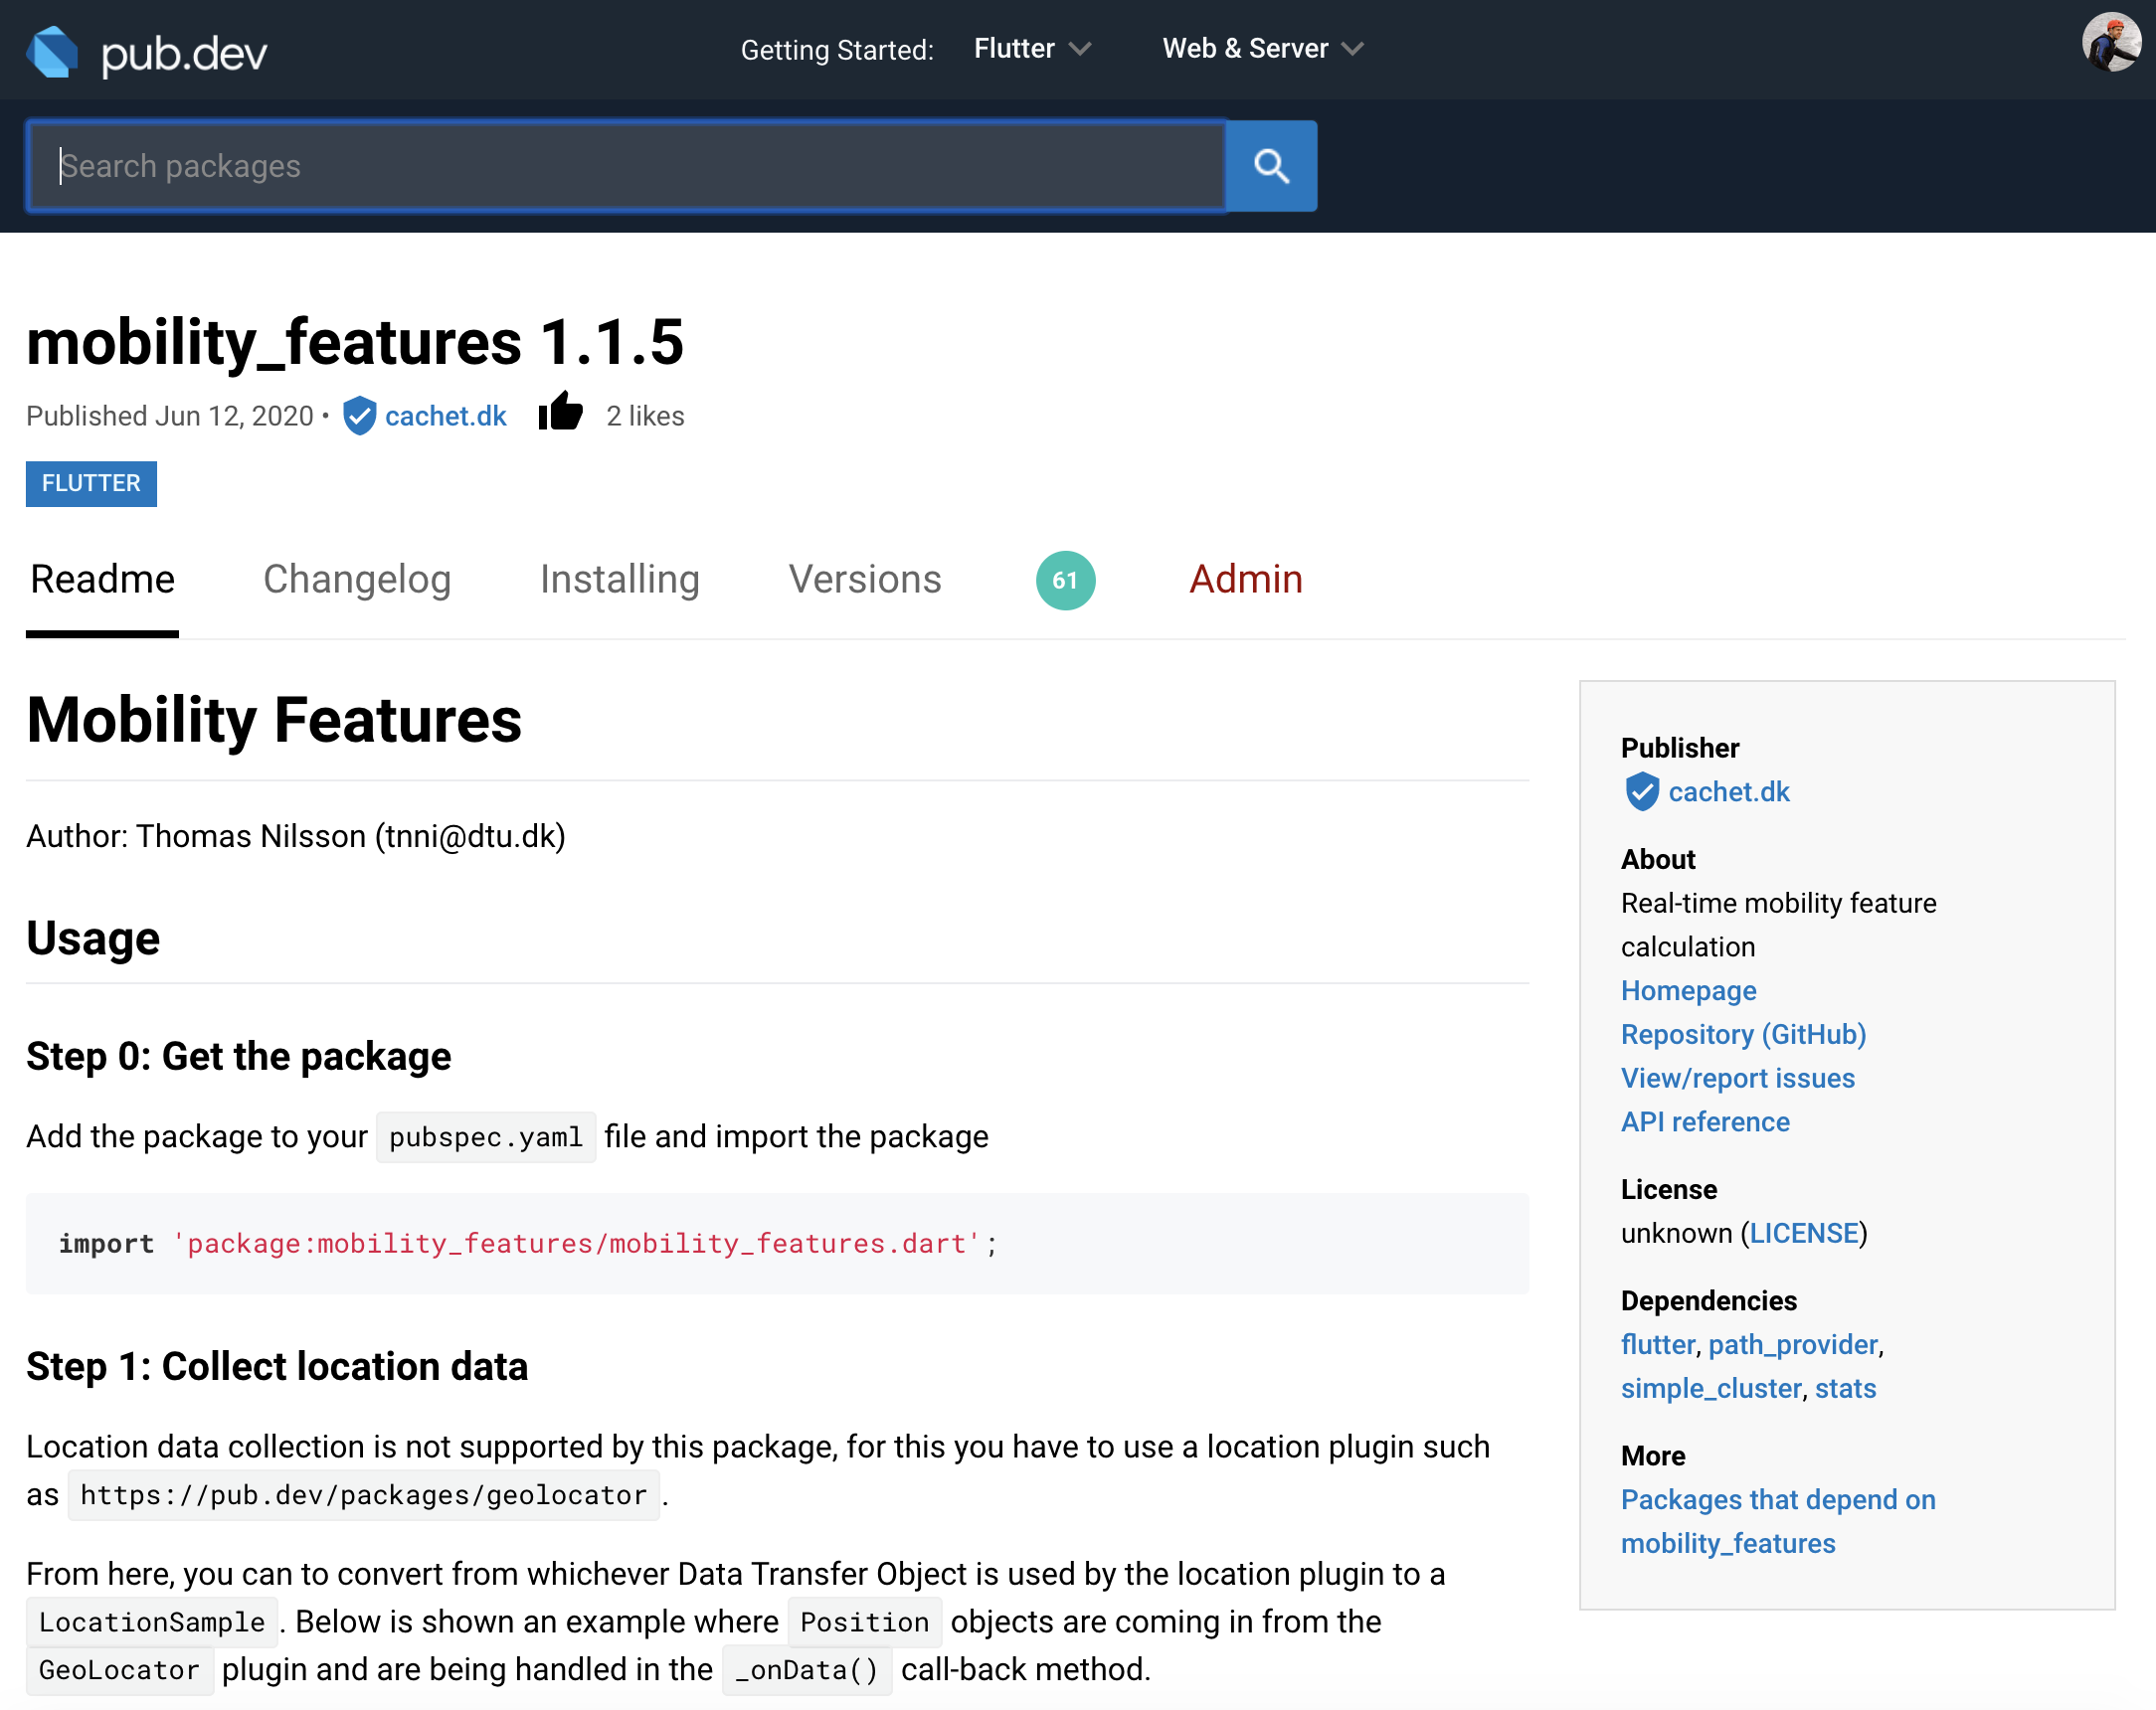
\includegraphics[width=\textwidth]{images/pub.png}
    \caption{The page hosting the Mobility Features Package on www.pub.dev}
    \label{fig:pub-package}
\end{figure}

Publishing automatically generate API documentation by using comments in the code. Normally, comments are made with 2 forward slashes (\textit{//}), but comments made with three forward slashes (\textit{///}) mark the code-block following it with API documentation, i.e. the contents of the comment. 

\begin{figure}
    \centering
    \begin{minted}{dart}
        /// A [LocationSample] holds a 2D [GeoPosition] spatial data point
        /// as well as a [DateTime] value s.t. it may be temporally ordered
        class LocationSample implements _Serializable, _Geospatial {...}
    \end{minted}
    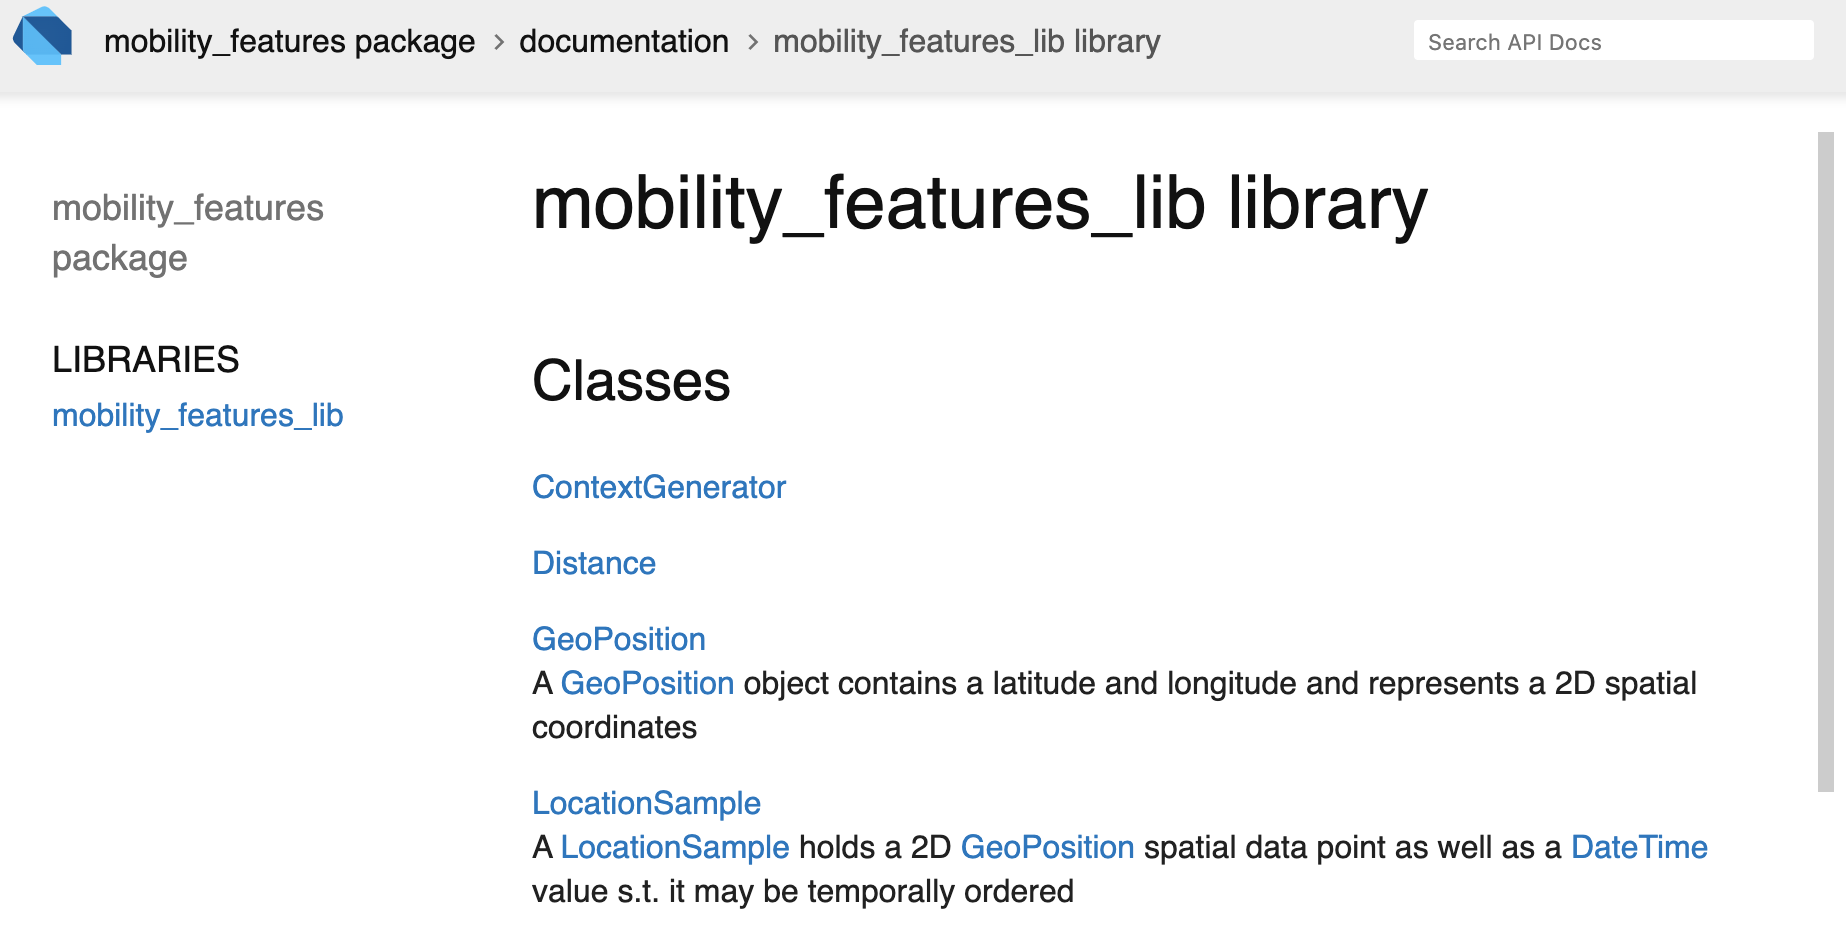
\includegraphics[width=\textwidth]{images/docs.png}
    \caption{The API comments for the source code of a Location Sample (top) and the auto generated documentation hosted on the Pub (bottom)}
    \label{fig:api-docs}
\end{figure}

